\documentclass{supervision}
\usepackage{course}

\Supervision{1}
\begin{document}
  \begin{questions}
    \section*{Search}
    \question Explain why breadth-first search is optimal if path-cost is a
      non-decreasing function of node- depth.

    \question In the graph search algorithm, assume a node is taken from the
      \lstinline|fringe| and found \textit{not} to be a goal and \textit{not} to
      be in \lstinline|closed|. We then add it to \lstinline|closed| and add its
      descendants to \lstinline|fringe|. Why do we not check the descendants
      first to see if they are in \lstinline|closed|?

    \question The $A^*$ algorithm does not perform a goal test on any state
      until it has selected it for expansion. We might consider a slightly
      different approach: namely, each time a node is expanded check all of its
      descendants to see if they include a goal.

      Give two reasons why this is a misguided idea, where possible illustrating
      your answer using a specific example of a search tree for which it would
      be problematic.

    \question The $f$-cost is defined in the usual way as:
      \begin{center}
        $f(n) = p(n) + h(n)$
      \end{center}

      where $n$ is any node, $p$ denotes path cost and $h$ denotes the
      heuristic. An admissible heuristic is one for which, for any $n$

      \begin{center}
        $h(n) \leq$ actual distance from $n$ to the goal
      \end{center}

      and a heuristic is monotonic if for consecutive nodes $n$ and $n'$ it is
      always the case that

      \begin{center}
        $f(n') \geq f(n)$.
      \end{center}

      \begin{parts}
        \part Prove that $h$ is monotonic if and only if it obeys the triangle
          inequality, which states that for any consecutive nodes $n$ and $n'$

          \begin{center}
            $h(h) \leq c_{n \rightarrow n'} + h(n')$
          \end{center}

        \part Prove that if a heuristic is monotonic then it is also admissible.

        \part Is the converse true? (That is, are all admissible heuristics also
          monotonic?) Either prove that this is the case or provide a
          counterexample.

      \end{parts}

    \question In RBFS we are replacing $f$ values every time we backtrack to
      explore the current best alternative. This seems to imply a need to
      remember the new $f$ values for all the nodes in the path we're
      discarding, and this in turn suggests a potentially exponential memory
      requirement. Why is this not the case?

    \section*{Games}

    \SetQuestionNumber{1}
    \question Consider the following game tree:
      \begin{center}
        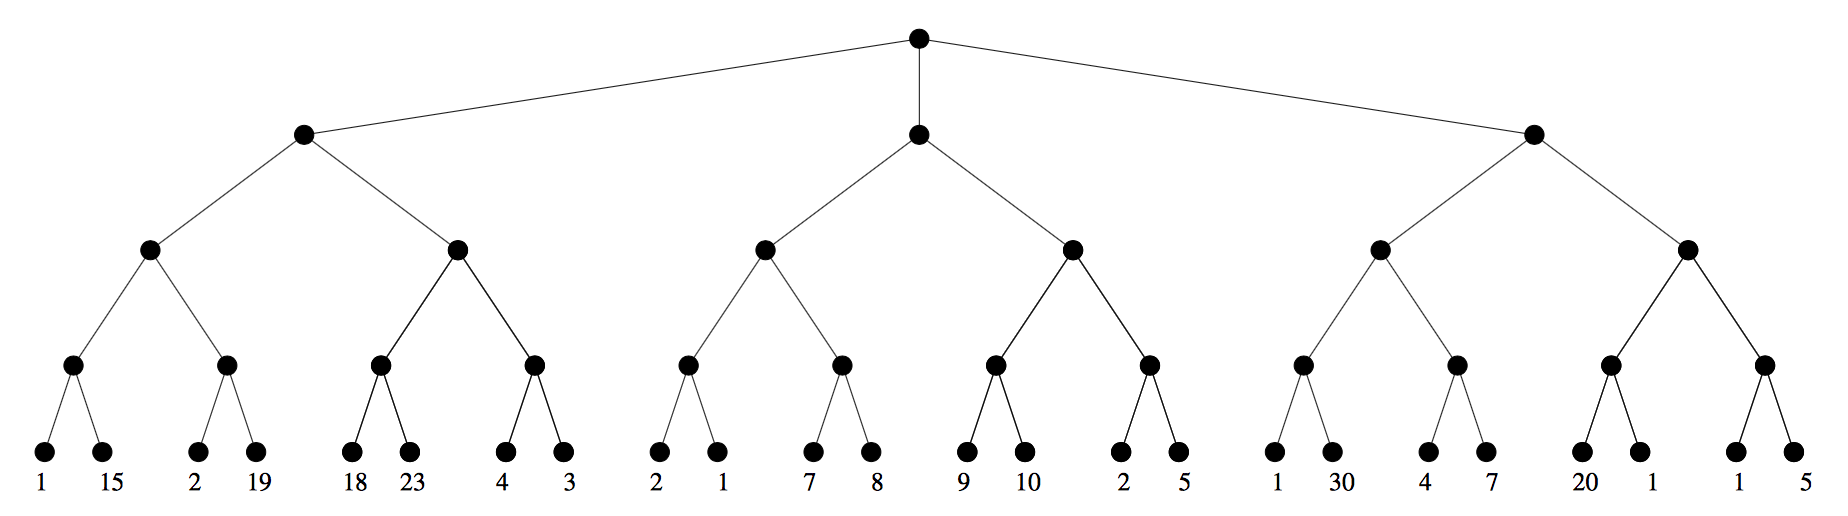
\includegraphics[width=0.9\textwidth]{1-graph}
      \end{center}

      Large outcomes are beneficial for Max. How is this tree pruned by $\alpha
      - \beta$ minimax if Max moves first? (That is, Max is the root.) How is it
      pruned if Min is the root, and therefore moves first?

    \question Implement the $\alpha - \beta$ pruning algorithm and use it to
      verify your answer to the previous problem.

    \question Is the minimax approach to playing games optimal against an
      imperfect opponent? Either prove this is the case or give a
      counterexample.

  \end{questions}
\end{document}
